% Preprocessing pipeline schematic (vector redraw of preprocessing_pipeline.jpg).
% Adds the stemming & stop-word step the old raster figure omitted (paper §3.5 step 5).
% Compile:  xelatex preprocessing_pipeline.tex
% Render :  pdftoppm -jpeg -r 600 -singlefile preprocessing_pipeline.pdf ../preprocessing_pipeline
\documentclass[border=6pt]{standalone}
\usepackage{helvet}\renewcommand{\familydefault}{\sfdefault}
\usepackage{tikz}
\usetikzlibrary{arrows.meta, positioning}
\begin{document}
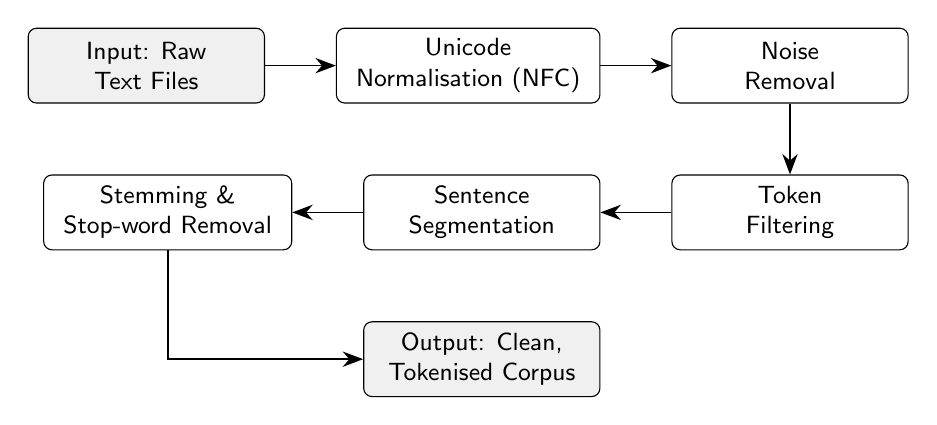
\begin{tikzpicture}[
  box/.style={draw, rounded corners=3pt, align=center, minimum height=9.5mm,
              minimum width=30mm, inner xsep=2.5mm, font=\small},
  io/.style={box, fill=black!6},
  arr/.style={-{Stealth[length=2.6mm]}, semithick}
]
  % top row, left to right
  \node[io]  (raw)   {Input: Raw\\Text Files};
  \node[box, right=9mm of raw]  (nfc)   {Unicode\\Normalisation (NFC)};
  \node[box, right=9mm of nfc]  (noise) {Noise\\Removal};
  % bottom row, right to left (snake)
  \node[box, below=9mm of noise] (tok)  {Token\\Filtering};
  \node[box, left=9mm of tok]   (sent)  {Sentence\\Segmentation};
  \node[box, left=9mm of sent]  (stem)  {Stemming \&\\Stop-word Removal};
  % output
  \node[io, below=9mm of sent]  (out)   {Output: Clean,\\Tokenised Corpus};

  \draw[arr] (raw)   -- (nfc);
  \draw[arr] (nfc)   -- (noise);
  \draw[arr] (noise) -- (tok);
  \draw[arr] (tok)   -- (sent);
  \draw[arr] (sent)  -- (stem);
  \draw[arr] (stem)  |- (out);
\end{tikzpicture}
\end{document}
